\documentclass[logo,dosguias,ejecucion]{tesis-pregrado}
% opciones: logo,dosguias,civil,ejecucion,propuesta,txfonts

\keywords{XML; Key Implication}

\begin{document}
\baselineskip 23pt
% ----------------------------------------------------------
% ----------- PARTE INICIAL --------------------------------
\thispagestyle{empty}
% Rellenar con la informacion personal y del trabajo

\titulo{Herramienta de dise\~no de objetos y visualizaci\'on de resultados para simulaci\'on de campo magn\'etico}

\autor{Juan Pablo Verdejo Jorquera}
\run{17190723-3}
\email{juan.verdejo@usach.cl}
\annoingreso{2015}

\fecha{Viernes}{05}{Junio}{2015}

\profesorguia{Fernando Rannou, Ph.D.}
\ciudad{Santiago}
\pais{Chile}

\makecubierta
\makecopyright % si es propuesta no se mostrará
% ----------------------------------------------------------
% ----------- PRIMERA PARTE --------------------------------
\frontmatter
% ### Resumen e Indices ####
% 
\begin{gracias}

\end{gracias}
% 
\dedicatoria{
  A mi\ldots
}

% 
\resumenCastellano{
La flexibilidad sintáctica, y el complejo anidamiento de los datos en una estructura tipo árbol 
dificulta expresar propiedades deseables de los datos XML, ofreciendo una capacidad limitada para 
expresar semántica. En esta tesis se presenta un estudio de las claves como restricciones de 
integridad sobre documentos XML, implementando algoritmos para los problemas de implicación y 
validación, con el fin de mostrar la factibilidad de usar las capacidades semánticas que éstas 
entregan, y que XML como modelo requiere.
\vspace*{0.5cm}
\KeywordsES{XML; Claves XML; Implicación de claves; Validación de documentos XML; Cover no redundante}
}

\newpage

\resumenIngles{
The syntactic flexibility and complex tree-like nested data make it challenging to express desirable 
properties of XML data, offering a limited capability to express semantic. In this thesis, we present 
a study of keys as integrity constraints on XML documents, implementing algorithms for implication 
and validation problems, with the aim of showing the factibility of using the semantic capabilities 
that keys gives and XML as a model requires.
\vspace*{0.5cm}
\KeywordsEN{XML; XML keys; Key implication; XML document validation; Non-redundant cover}
}

\pagestyle{fancy}
\fancyhead[L]{\slshape \leftmark}
\fancyhead[C]{}
\fancyhead[R]{\thepage}
\tableofcontents        %% Indice general
\listoffigures          %% Indice de figuras
\listoftables           %% Indice de tablas
\listofalgorithms       %% Indice de algoritmos
% ----------------------------------------------------------
% ----------- SEGUNDA PARTE --------------------------------
\mainmatter
% ### Configuración del header ###
\pagestyle{fancy}
\fancyhead[L]{\slshape \leftmark}
\fancyhead[C]{}
\fancyhead[R]{\thepage}
\pagenumbering{arabic}
% ### Capitulos de la tesis ###
\chapter{Introducci\'on}
\label{cap:intro}

\section{Antecedentes y motivaci\'on}
\label{intro:motivacion}

Un grupo de científicos del Departamento de Física de la Universidad de Santiago de Chile trabaja en la simulación de los efectos del campo magnético en los átomos de distintos objetos, tomando en cuenta su forma, su material y su distribución atómica, entre otras características, usando una aplicación escrita en C empleando el Método de Monte Carlo \citep{MonteCarlo}.

No obstante lo anterior, uno de los grandes problemas de los científicos es que el proceso previo y posterior a la simulación es ``manual'', para definir el objeto deben hacer un dibujo en Microsoft Paint\textregistered, el cual es analizado por un \emph{script} de Matlab\textregistered\ que debe ser modificado para reflejar las características del objeto en específico que se quiere simular. Para generar imágenes para, por ejemplo, una publicación, también deben ejecutar ciertos \emph{scripts}, sin embargo esto es aún más complicado, ya que deben hacer ensayo y error hasta conseguir que la imagen sea representativa del resultado, puesto que muchas veces tienen errores de visualización que no reflejan el estado real. Estos dos sub-procesos hacen que el proceso de simulación sea tedioso, quitando mucho tiempo que podría ser usado en analizar los resultados.

Es aquí donde la informática puede contribuir, creando aplicaciones que mejoren estos procesos, que valoricen el tiempo de los científicos. Por consiguiente esta es una oportunidad única de ayudar a la obtención de conocimientos que permitan entender el entorno y de mejorar los procesos que permiten avanzar como sociedad hacia la comprensión del universo.


\section{Descripci\'on del problema}
\label{intro:problema}

Los científicos no disponen de una herramienta automatizada de diseño de objetos para aplicar la simulación MonteCarlo, que permita definir características físicas y geométricas y crear un archivo de entrada, que describa cada uno de los átomos, para la simulación, la cual es hecha por un software escrito en C por un anterior tesista del Departamento. Además se necesita que la herramienta permita mejorar el proceso de análisis y publicación de los resultados entregados por esta simulación.

\section{Estado del arte}

\subsection{Proceso actual}
Actualmente los investigadores deben preparar la simulación usando un \emph{script} en Matlab\textregistered, el cual analiza un archivo \emph{.bmp} creado en \emph{Microsoft Paint\textregistered}, esta imagen generalmente es pequeña, menor a 50px x 50px, y representa la primera capa del objeto (mirado desde arriba), para esto se marcan los pixeles que describen el objeto, de esta forma el mapa de \emph{bits} es binario, si un \emph{pixel} es negro se considera un 1, si es blanco se considera un 0. En este \emph{script} se describen características específicas del objeto que se quiere definir, entre ellos:
\begin{itemize}
	\item Número de capas: Cuantas veces se repite la primera capa para formar un objeto en 3D.
	\item Distribución de los átomos (ver anexo A): Como premisa se trabaja sólo con distribuciones cúbicas de átomos, no obstante estas distribuciones tienen ciertas características específicas, por ejemplo:
	\begin{itemize}
		\item Cúbico simple (SC por \emph{Simple Cubic}): En cada vértice de una distribución cúbica se encuentra un átomo.
		\item Centrado en las caras (FCC por \emph{Face-centered Cubic}): Además del átomo en cada vértice de la distribución cúbica, hay un átomo en el centro de cada cara de la distribución.
		\item Centrado (BCC por \emph{Body-centered Cubic}):  Además del átomo en cada vértice de la distribución cúbica, hay un átomo en el centro de cada distribución.
	\end{itemize}
	\item Coeficiente de escalamiento: Es un coeficiente usado para dar al objeto las medidas deseadas para ejecutar la simulación.
\end{itemize}

Este proceso produce un archivo de texto plano describiendo cada uno de los átomos del objeto sobre el cuál se aplicará la simulación.

Luego de ejecutada la simulación el software entrega múltiples archivos de texto, uno que define cada uno de los átomos con un ID y una posición en el espacio, y N archivos que definen la fuerza magnética de cada átomo en un tiempo dado. Los científicos deben seleccionar uno de estos archivos y aplicar un \emph{script} de Matlab\textregistered\ para poder visualizar el resultado.

El proceso de exportación de imágenes para publicaciones puede tomar un día de trabajo para los científicos, ya que deben hacer ``ensayo y error'' hasta que la imagen producida refleje lo que desean. Luego deben esperar por la aprobación por parte del profesor guía, en caso de ser rechazada, deben volver a ejecutar el proceso.

\subsection{Soluciones similares}
Existe una herramienta que hace simulaciones similares a las que hace el grupo de científicos llamada ``Go Parallel Magnet\textregistered''. A pesar de que la simulación no es exactamente la misma, el flujo de diseño es útil para el proyecto. Sin ir más lejos los científicos basan el proceso actual en éste.

``Go Parallel Magnet\textregistered'' usa para el diseño un sistema de multi-capas, donde se define la capa superior del objeto y se indica la cantidad de veces que ésta se repetirá. Con estos datos se crea un objeto en 3D que luego se transforma en la estructura molecular deseada.

\section{Propósitos de la solución}
\begin{enumerate}
  \item Mejorar el proceso de preparación de la simulación.
  \item Mejorar el proceso de exportación de imágenes para publicaciones.
\end{enumerate}


\section{Alcances o limitaciones de la solución}
\begin{itemize}
	\item El software se encargará del diseño de objetos para la simulación entregando la entrada para ésta y posteriormente de la visualización de los resultados, y de la exportación de estos para publicaciones, mas \textbf{NO} se encargará de la simulación en sí y queda fuera del alcance de la solución.
	\item La aplicación estará disponible para sistema operativo MAC OS X.
	\item El diseño de objeto será por capas, es decir, se define la ``vista superior'' y la cantidad de veces que se repetirá hacia abajo.
\end{itemize}

\section{Objetivos y alcance del proyecto}
\label{intro:objetivos}

\subsection{Objetivo general}
Crear un software que permita diseñar objetos en 3D, con características físicas y geométricas específicas, sobre los cuáles se aplicarán simulaciones de campo magnético a nivel atómico y analizar los resultados de forma visual, permitiendo la exportación de imágenes para publicaciones.

\subsection{Objetivos espec\'ificos}

Para la consecución del objetivo general, se plantean las siguientes metas intermedias para el software:

\begin{enumerate}
  \item Modelar el proceso de simulación del efecto de campo magnético en átomos efectuado por los científicos del Departamento de Física de la Universidad de Santiago de Chile.
  \item Diseñar la herramienta informática de ayuda para la investigación antes mencionada.
  \item Crear el software.
  \item Validar el cumplimiento de los requerimientos.
\end{enumerate}


\section{Características de la solución}

Como solución se propone la creación de un software que facilite el trabajo de los científicos. Esta aplicación se divide en dos funcionalidades:

\subsection{Diseño del objeto sobre el cuál se hará la solución:}

El software debe permitir crear visualmente un objeto en 3D, con ciertas características físicas como la distribución cúbica (ver anexo A). Luego de la creación y configuración del objeto la aplicación debe exportar un archivo de texto que sirva como entrada para el software que hará la simulación. Este archivo tiene un formato ya definido y debe describir la posición de cada átomo del objeto.

Este proceso se divide en tres características:

\begin{enumerate}
	\item Creación de objeto en base a un mapa de \emph{bits} binario, con características pre-definidas, y exportación de archivo de entrada para la simulación.
	\item Permitir la entrada de características del objeto, como número de capas y ordenamiento de los átomos.
	\item Visualización atómica en 3D del objeto sobre el cuál se hará la simulación.
\end{enumerate}

\subsection{Visualización de resultados de la simulación:}

El software debe tomar la totalidad de archivos de salida de la simulación como entrada y debe ser capaz de mostrar visualmente el estado magnético de cada átomo en un tiempo \emph{t}, también debe ser posible ver la simulación animada a través del tiempo, como un video.

La salida de la visualización serán imágenes en 2D del estado de la simulación en un tiempo \emph{t}, estas imágenes deben tener colores que permitan al lector entender el resultado a pesar de la dimensión faltante, por ejemplo, usando la proyección del vector en uno de los ejes y asignando un color según la intensidad de éste.

Este proceso se divide en tres características:

\begin{enumerate}
	\item Permitir ver el estado de la simulación en 3D en un tiempo \emph{t}.
	\item Permitir ver el cambio de estado de la simulación en 3D de forma animada.
	\item Permitir exportar el estado de la simulación en un tiempo \emph{t} en 2D para publicaciones.
\end{enumerate}


\section{Propósitos de la solución}
\begin{enumerate}
  \item Mejorar el proceso de preparación de la simulación.
  \item Mejorar el proceso de exportación de imágenes para publicaciones.
\end{enumerate}


\section{Alcances o limitaciones de la solución}
\begin{itemize}
	\item El software se encargará del diseño de objetos para la simulación entregando la entrada para ésta y posteriormente de la visualización de los resultados, y de la exportación de estos para publicaciones, mas \textbf{NO} se encargará de la simulación en sí y queda fuera del alcance de la solución.
	\item La aplicación estará disponible para sistema operativo MAC OS X.
	\item El diseño de objeto será por capas, es decir, se define la ``vista superior'' y la cantidad de veces que se repetirá hacia abajo.
\end{itemize}


\section{Metodolog\'ia y herramientas utilizadas}
\label{intro:metodologia}

\subsection{Metodolog\'ia}
Dado que se tiene conocimiento de los requerimientos mayores, pero pueden existir detalles al trabajar en un ámbito tan específico como simulaciones físicas, se decidió usar una modificación de Scrum \citep{SCRUM}.

Scrum está pensado para trabajar en equipos con varios desarrolladores, además de los cargos más de gestión, para esto se tienen 3 roles \citep{website:ScrumRoles}:

\begin{description}
  \item[\emph{Product Owner}] \hfill \\
  Es el encargado de maximizar el valor del trabajo el equipo, para esto tiene un alto conocimiento del producto mediante un contacto directo con los \emph{stakeholders} y facilita la comunicación de estos con el equipo de desarrollo, debido a esto es el responsable de decidir qué se va a construir, pero no el cómo. Para este proyecto el \emph{Product Owner} será el profesor Fernando Rannou, quién tiene contacto constante con los \emph{stakeholders} por proyectos paralelos que se están desarrollando.
  \item[\emph{Scrum Master}] \hfill \\
  Es el líder del equipo de desarrollo y debe tener un buen conocimiento de la metodología scrum, el cual debe traspasar al equipo de desarrolladores. Sus 3 principales tareas son: Guíar al equipo teniendo un conocimiento tanto del producto como de las tecnologías a utilizar, mantener al equipo avanzando eliminando toda dificultad que puedan tener durante el desarrollo, estas dificultades pueden ser tanto internas como externas, y enseñar a metodología \emph{scrum} al equipo. En este caso como solo un desarrollador trabajará en el proyecto y este tiene un gran conocimiento de la metodología gracias a sus años de experiencia laboral usandola, no se usará este rol.
  \item[Desarrollador] \hfill \\
  El desarrollador es el encargado de entregar los incrementales del producto, para eso se basa en la lista de tareas definidas por el \emph{Product Owner} al inicio de un \emph{sprint}. En este proyecto solo trabajará un programador.
\end{description}

Otras modificaciones hechas a la metodología fue modificar alguna de sus ceremonias, cambiando la reunión diaria (\emph{Daily Scrum}) por una semanal, entre el profesor y el desarrollador, las reuniones retrospectivas al finalizar cada \emph{sprint} se unió con la de planificación del siguiente periodo de desarrollo. Además, como es recomendado, se tuvo una reunión con los \emph{stakeholders} luego de cada sprint.

Estas modificaciones fueron necesarias para poder usar la metodología en un proyecto con solo un desarrollador y optimizando al máximo el tiempo usado en reuniones, debido al poco espacio en las agendas tanto del desarrollador como del \emph{Product Owner}.

\subsection{Herramientas de desarrollo}
\subsection{Modelado 3D: OpenGL}
Se usará OpenGL como biblioteca de modelado 3D, por ser el estado del arte en este ámbito, entre sus ventajas está el ser multi-plataforma, lo que eventualmente permitiría una rápida portación a otro sistema operativo, y el ser la más usada actualmente, lo que permite que tenga una amplia comunidad de usuarios que la soportan y documentan.

\subsection{Lenguaje de programación: Python}
Para el desarrollo se usará el lenguaje de programación Python con la biblioteca wxPython para Intefaz de Usuario. Esta biblioteca tiene soporte para la API OpenGL. Python, al ser un lenguaje multiplataforma, permitiría una rápida portación a otro sistema operativo en el futuro.

\subsection{Control de versiones: GIT}
Para el versionamiento del código se usará GIT, manteniendo un respaldo del repositorio con el código y la documentación en una máquina virtual con Linux ubicada en Estados Unidos.

\section{Ambiente de desarrollo}
Para el desarrollo se usará el siguiente ambiente de desarrollo:
\begin{itemize}
	\item Computador marca Apple, con una tarjeta gráfica que soporte OpenGL 3.2+ y sistema operativo Mac OS X para el desarrollo.
	\item Una máquina virtual con Linux, ubicada en Estados Unidos, para mantener un respaldo del código y de la documentación.
\end{itemize}

\chapter{Arquitectura de la solución}
\label{cap:arquitectura}


\section{Clases}

Para el desarrollo de la aplicación se usó el lenguaje Python, dividiendo la aplicación en clases que se pueden categorizar de la siguiente forma:

\subsection{Clases visuales}

\subsubsection{MolDesigner}
Esta es la clase principal del programa, ya que es la encargada de iniciar el programa, cargando todas las dependencias necesarias para su ejecución, pero principalmente tiene la lógica de la parte visual del \emph{software}, es decir, de la creación y distribución en pantalla de los distintos elementos visuales, como ventanas, botones, campos de texto, etc., además de la interacción del usuario con estos. Cada reacción a una acción ejecutada sobre estos elementos es orquestada por esta clase.

\subsubsection{BitmapGrid}
La clase BitmapGrid es la encargada de manejar la grilla con la cuales los cientificos diseñarán los objetos sobre los cuales se simulará, para esto se basa en la biblioteca \emph{wx.grid} de \emph{wxPython}, una implementación de una planilla de cálculos tipo \emph{excel}, la cual es modificada para no poder ser editada y que las distintas acciones del \emph{mouse} sobre esta (click, seleccionar fila o columna, seleccionar un rango de celdas, etc.) generen cambios en el color de fondo de cada celda, pudiendo este ser negro o blanco, transformando esta planilla de cálculos en un mapa de bits binario.

Entre las características de este mapa de bits se encuentra la capacidad de crear figuras predefinidas rápidamente, por ejemplo, se puede dibujar un cuadrilátero indicando el ancho, el alto y seleccionando la esquina superior derecha de esta figura. También es posible crear un círculo indicando el radio que tendrá este y su centro.

\begin{figure}[H]
  \centering
  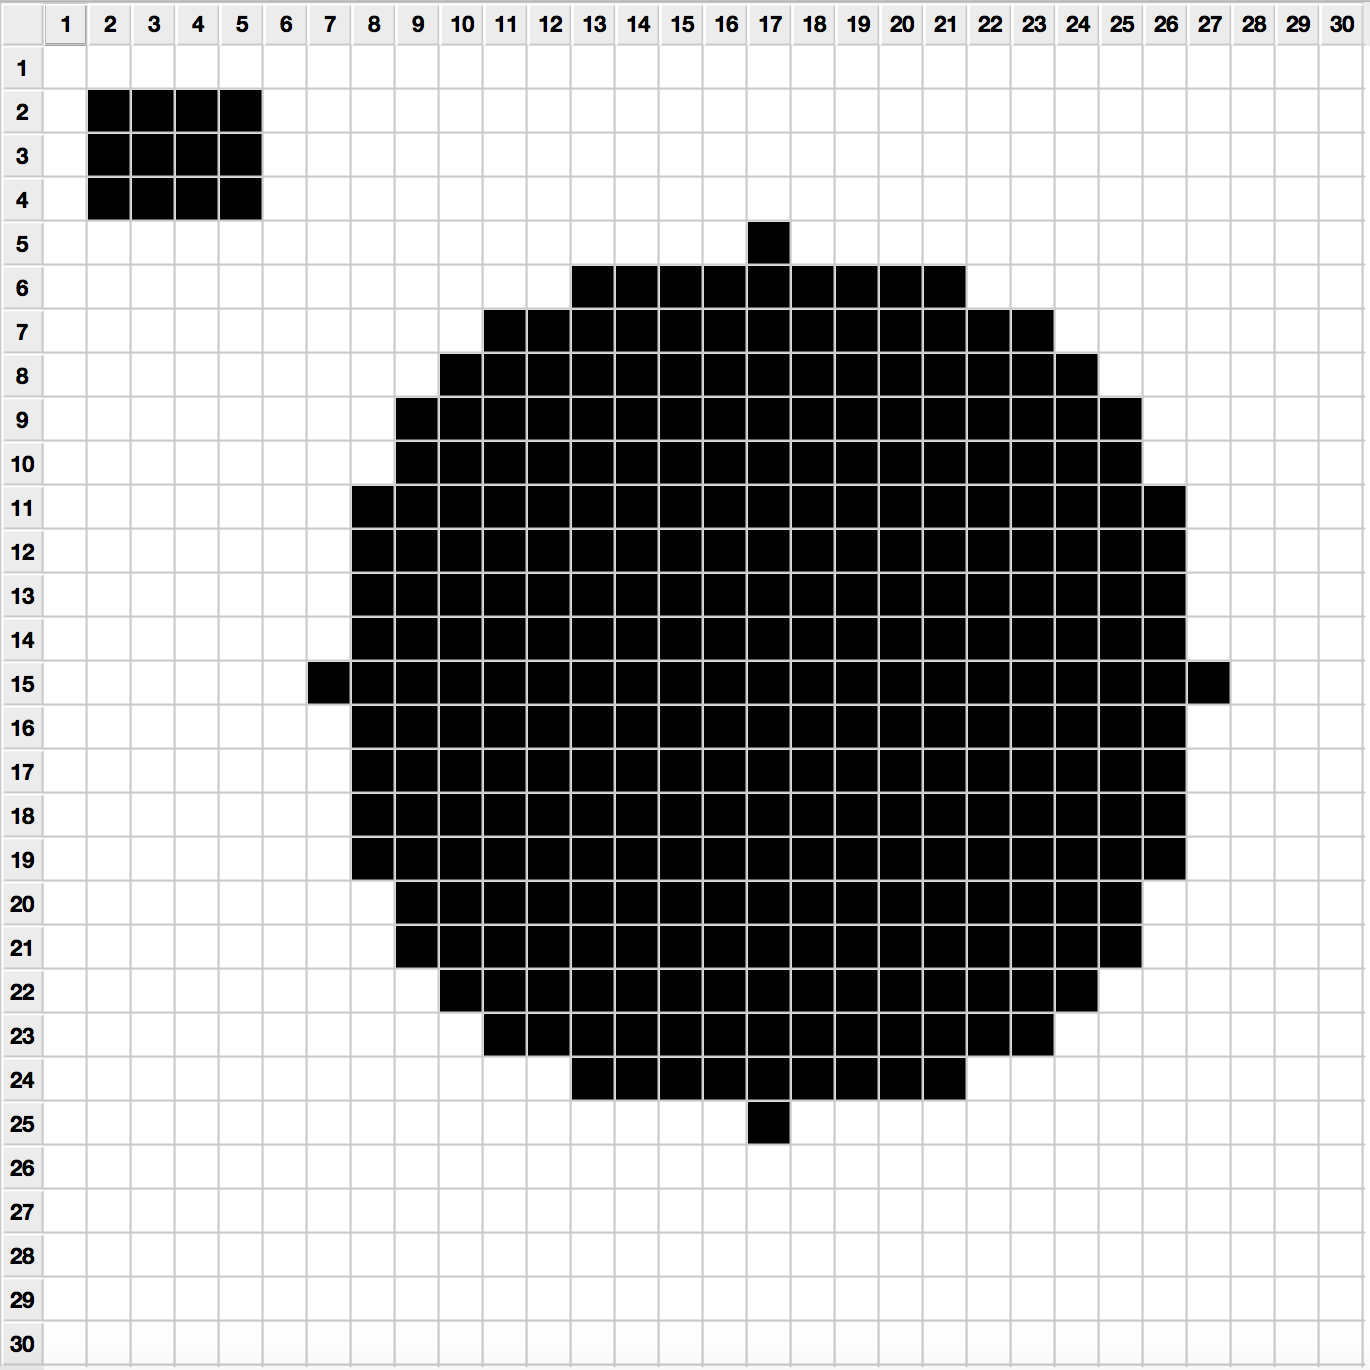
\includegraphics[scale=.5]{images/bitmapGrid}
  \caption{\em Mapa de bits binario con 2 figuras pre-diseñadas.}
\end{figure}

\subsection{Clases 3D}

Estas clases son las encargadas de manejar los distintos \emph{canvas} que se usan en el \emph{software}, tanto para la visualización del diseño y del resultado de la simulación, como para ayudas referenciales para los científicos.

\subsubsection{AtomCanvas}

La clase AtomCanvas es la más importante con respecto a la visualización 3D, ya que es la encargada de mostrar en pantalla tanto el diseño de los objetos sobre los cuales se correrá la simulación como los resultados de estas usando OpenGL. En el desarrollo de esta se puso énfasis en la optimización, pudiendo mostrar sin mayores demoras más de 20.000 átomos, para tener una idea un sistema promedio analizado por los científicos usa 3.000 átomos (TODO: CONFIRMAR).

Otra de las tareas de esta clase es manejar las distintas interacciones del usuario, tanto con el teclado como con el \emph{mouse} con las representaciones en 3D, como rotaciones, movimientos y \emph{zoom}.

Para la visualización del diseño se usan esferas de distintos colores, representando cada uno de los distintos tipos de átomos que pueden haber según la estructura cúbica elegida. En las siguientes imágenes se representan una estructura de 5x5, con 3 capas, siendo solo diferente la estructura cúbica elegida.

\begin{figure}[H]
  \centering
  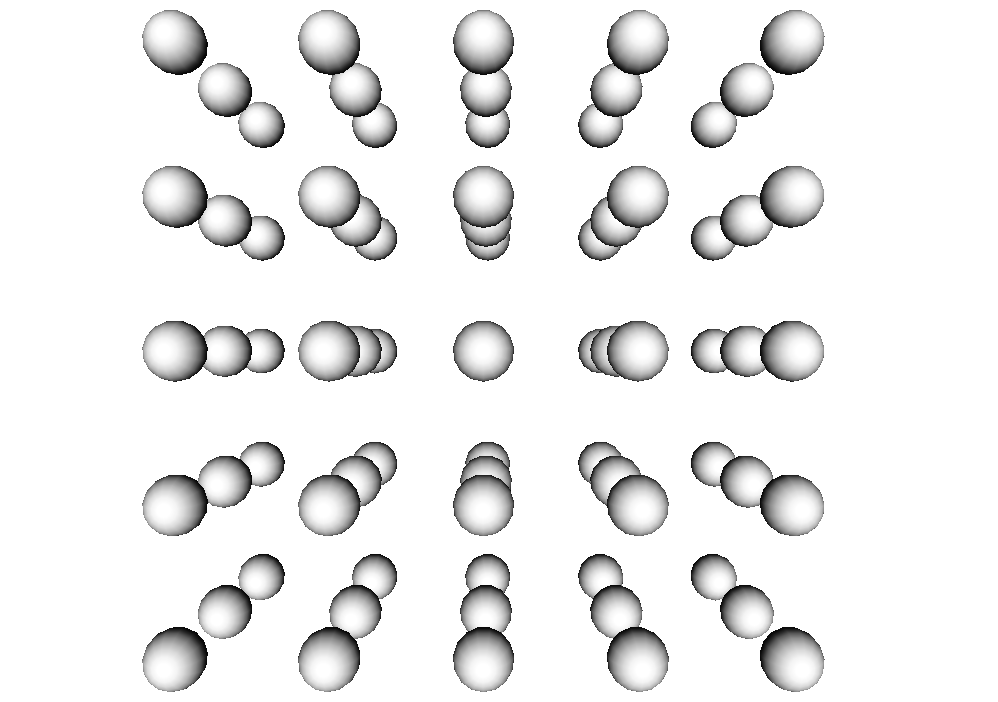
\includegraphics[scale=.3]{images/atomCanvas-SC}
  \caption{\em En un SC todos los átomos son blancos.}
\end{figure}

\begin{figure}[H]
  \centering
  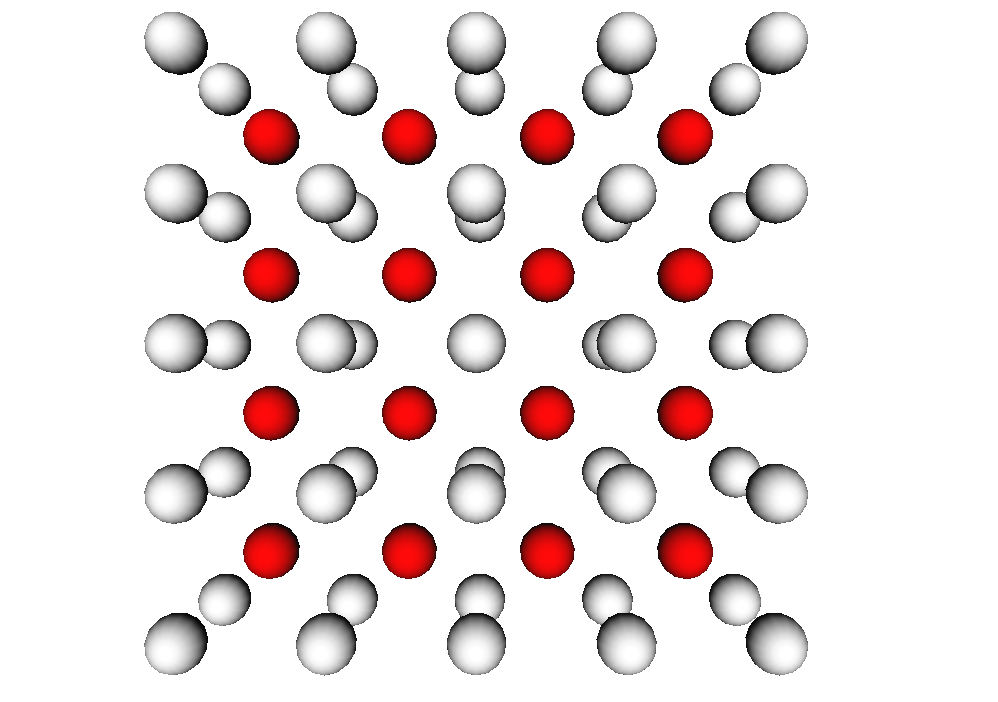
\includegraphics[scale=.3]{images/atomCanvas-BCC}
  \caption{\em En un BCC los átomos centrales son rojos.}
\end{figure}

\begin{figure}[H]
  \centering
  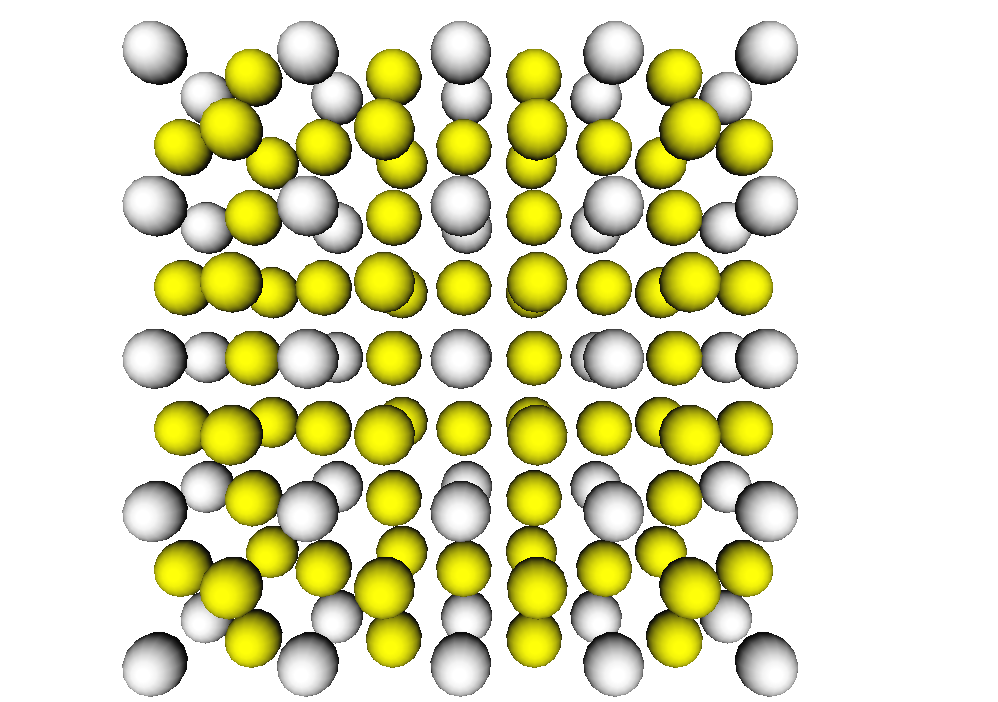
\includegraphics[scale=.35]{images/atomCanvas-FCC}
  \caption{\em En un FCC los átomos de las caras son amarillos.}
\end{figure}

En el caso de la visualización de resultados se usan flechas de colores como representación. Para asignar un color a una flecha se parte de la premisa que en tiempo t=0 el campo magnético está cargado hacia un eje, es decir, todos los vectores serán iguales, teniendo la misma magnitud, sentido y dirección, estando este paralelo a uno de los ejes del plano coordenado; además se sabe que en ese momento su magnitud es máxima. Si inicialmente todos los vectores son paralelos al eje A, se usará la componente â de cada vector para definir el color, si la componente es 0 será de color verde, si la magnitud es máxima en sentido contrario a los vectores iniciales el color será azul, si la magnitud es máxima en el mismo sentido de los vectores iniciales el color será rojo. Como se puede inferir la escala va desde azul a rojo, siendo este último color el inicial para todos los vectores.

\begin{figure}[H]
  \centering
  
\includegraphics[scale=.5]{images/atomCanvas-colorScale}
  \caption{\em Escala de colores de azul a rojo.}
\end{figure}

\begin{figure}[H]
  \centering
  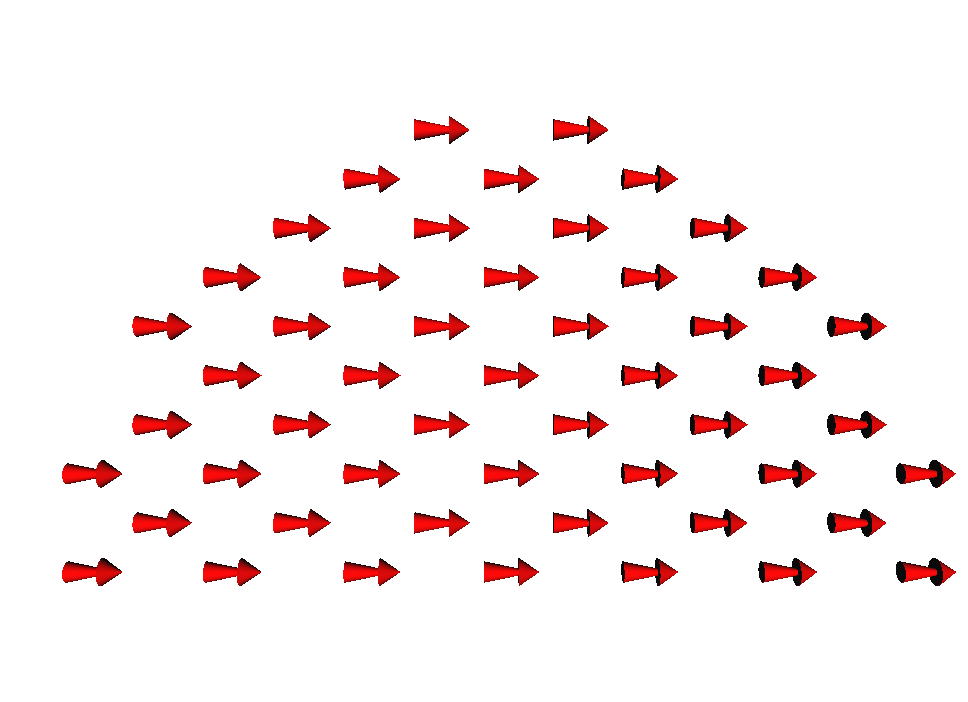
\includegraphics[scale=.3]{images/atomCanvas-vectores-inicial}
  \caption{\em Estado inicial de la visualización, con todos los vectores rojos cargados al eje X.}
\end{figure}

\begin{figure}[H]
  \centering
  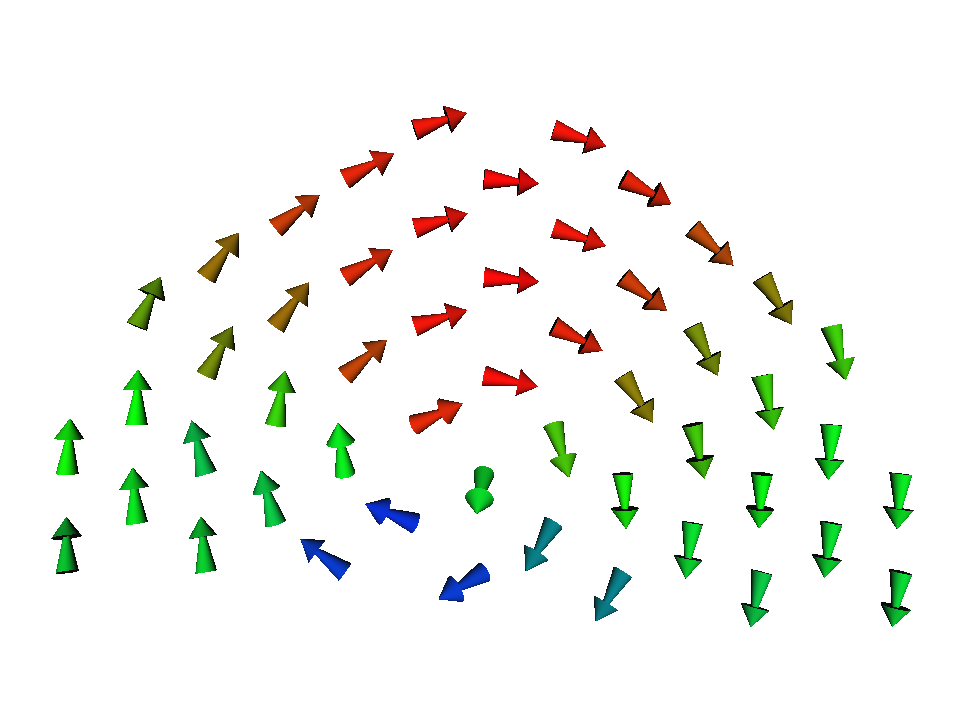
\includegraphics[scale=.3]{images/atomCanvas-vectores-colores}
  \caption{\em Vectores de distintos colores segun la componente î.}
\end{figure}

\subsubsection{Axes}

La clase Axes es la encargada de mostrar los ejes coordenados de los distintos canvas, tanto del de diseño de objetos como el de visualización de resultados, usando Open GL.
Cada eje se representa con su propio color, usando azul, rojo y verde para los ejes X, Y y Z respectivamente, y una etiqueta con el mismo color, de forma de hacerlo fácil de visualizar para el usuario.
Debido al diseño del \emph{software}, donde las distintas funciones del programa (diseño y visualización) se seleccionan mediante pestañas, esta clase debe ser instanciada 2 veces, ya que no es posible usar la misma instancia en ambas secciones. Estas se comunican directamente con AtomCanvas para obtener los distintos parametros de rotación de forma que los ejes sean coherentes a la imagen mostrada.

\begin{figure}[H]
  \centering
  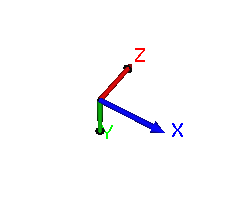
\includegraphics[scale=1]{images/axes}
  \caption{\em Representación visual de los ejes coordenados.}
\end{figure}

\subsection{Clases de cubos}

Las clases de cubos son 3 clases hermanas que calculan los átomos de un objeto que se está diseñando, todas tienen solo 2 métodos: \emph{calculate} y \emph{find\_neighborhood}, el primero se encarga de identificar todos los átomos que aplican dados los parametros físicos como la estructura de la primera capa, luego el segundo busca, para cada átomo, todos sus vecinos inmediatos, estos parametros son necesarios para exportar el archivo que luego servirá de entrada para la simulación.

\subsubsection{SC}
SC es la clase que maneja los cubos simples (\emph{Simple Cubic} o \emph{SC}), estas estructuras cúbicas se caracterizan por tener un átomo en cada uno de sus vértices, por lo que el cálculo de sus átomos se reduce a simplemente repetir la capa superior tantas veces como sea indicado en la entrada de propiedades físicas. Para encontrar el vecindario es necesario buscar todos los átomos que estén en las siguientes posiciones relativas [-1,0,0], [1,0,0], [0,-1,0], [0,1,0], [0,0,-1] y [0,0,1], por lo que el tamaño máximo de su vecindad es de 6 átomos.

\subsubsection{BCC}
BCC es la clase que maneja los cubos centrados en el cuerpo (\emph{Body Centered Cubic} o \emph{BCC}), que son las estructuras cúbicas que además de tener un átomo en cada vértice de los cubos tienen uno en el centro de cada uno de estos, de tal forma que en el cálculo de átomos se debe trabajar con una capa intermedia que contendrá los centros de cada cubo, de tal forma que para una estructura de 5 capas quedaría así:
\begin{center}
  \begin{tabular}{ c | l }
    \# & Capa \\
    \hline
    1 & Primaria \\
    2 & Intermedia \\
    3 & Primaria \\
    4 & Intermedia \\
    5 & Primaria \\
    \hline
  \end{tabular}
\end{center}

La regla para agregar un átomo central es que debe tener un cubo de átomos a su alrededor, en caso de que el cubo no esté completo simplemente se usarán las capas primarias:

\begin{figure}[H]
  \centering
  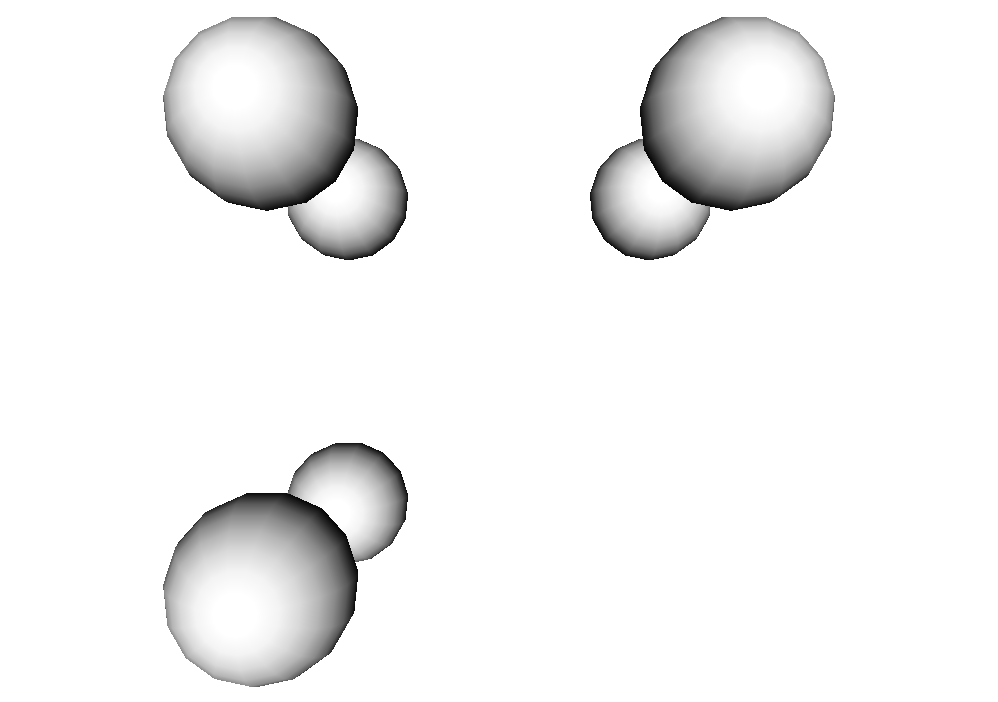
\includegraphics[scale=.3]{images/BCC-incomplete-molecule}
  \caption{\em Cubo BCC incompleto, sin átomo central}
\end{figure}

\begin{figure}[H]
  \centering
  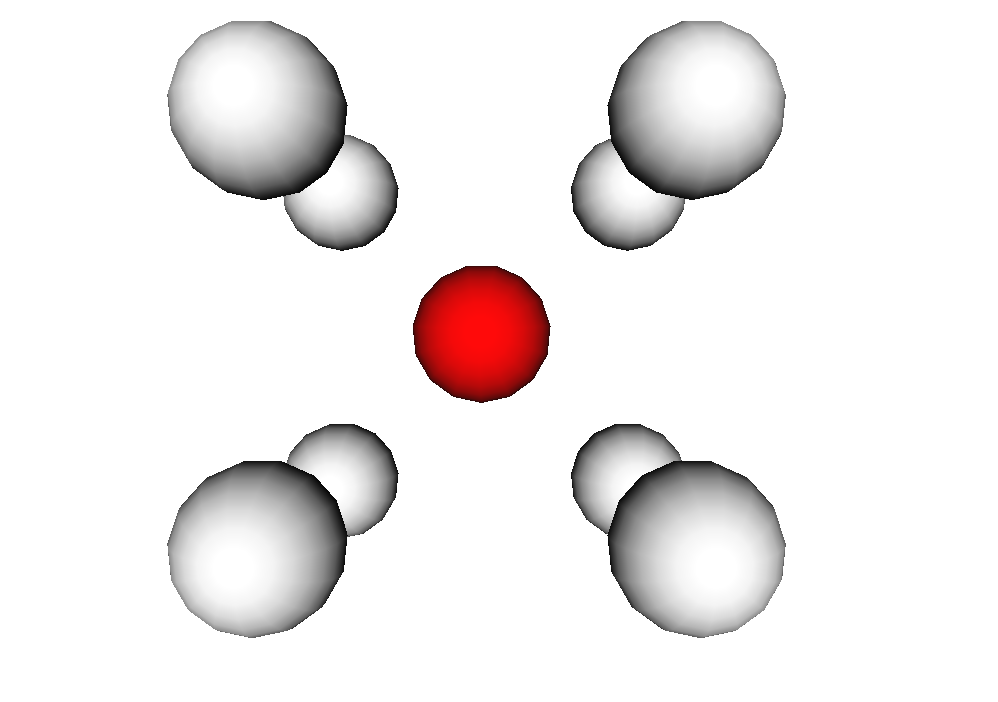
\includegraphics[scale=.3]{images/BCC-complete-molecule}
  \caption{\em Cubo BCC completo, con átomo central}
\end{figure}

En el caso de los BCC los átomos que conforman la vecindad siempre estarán en las posiciones relativas $[\pm 0.5, \pm 0.5, \pm 0.5]$, es decir, cada átomo puede tener una vecindad compuesta por hasta 8 átomos.

\subsubsection{FCC}
FCC es la clase que maneja los cubos centrados en las caras (\emph{Face Centered Cubic} o \emph{FCC}), los cuales se caracterizan por tener un átomo extra por cara además de uno en cada uno de sus vertices, por lo que además de tener que crear una capa intermedia es necesario modificar la capa primaria, es decir, la que crea el usuario usando el mapa de bits. La regla para agregar estos átomos en las caras es que esté en la diagonal creada por otros 2 átomos, en cualquier dirección. En la siguiente imagen se ve una estructura cúbica de 1x2, como en una de sus caras se forma una diagonal entre 2 átomos se agrega uno extra en una capa intermedia.

\begin{figure}[H]
  \centering
  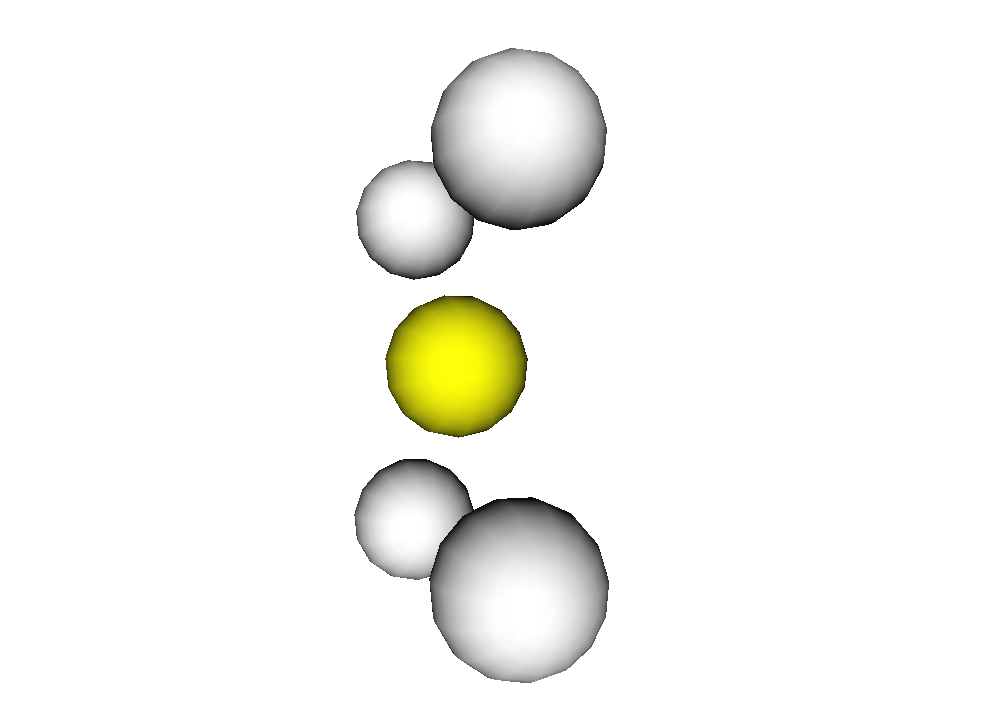
\includegraphics[scale=.3]{images/FCC-diagonal}
  \caption{\em Estructura cúbica FCC, con átomo en una de sus caras}
\end{figure}

La vecindad de estas estructuras cúbicas está dada por la posición relativa dada por $[\alpha, \beta, \gamma]$, donde:

$ (\alpha = \pm 0.5; \beta = \pm 0.5; \gamma = 0) \vee (\alpha = \pm 0.5; \beta = 0; \gamma = \pm 0.5) \vee (\alpha = 0; \beta = \pm 0.5; \gamma = \pm 0.5)$

Lo que en su combinatoria resulta 12 posiciones, siendo este el número máximo de átomos en una vecindad.


% ----------------------------------------------------------
% ----------- TERCERA PARTE --------------------------------
% \backmatter %Elimina la numeración
% ### Bibliografía de este documento ###
\bibliographystyle{apa-good}
\bibliography{referencias}
% ----------------------------------------------------------
% ----------- CUARTA PARTE ---------------------------------
\appendix
\addappheadtotoc %agregar Apéndice al índice. Si no tiene apéndices COMENTAR o BORRAR
% \noappendicestocpagenum %quitar número de páginas a los apéndices
% ### ANEXOS ###
% 
\chapter{Manual de usuario}
\label{cap:manual}

%DESCOMENTAR ESTAS LINEAS SI EL CAPÍTULO TIENE FIGURAS O TABLAS
%\addtocontents{lof}{{\bf \noindent Figuras del Anexo \Alph{chapter}}}
\addtocontents{lot}{{\bf \noindent Tablas del Anexo \Alph{chapter}}}

\section{Requerimientos previos}

\subsection{Requerimientos para instalación}
blablabla

\begin{table}[ht]
\caption{Tabla que dice nada}\label{tab:nombreTablaReferenciable}
\small %hace que el contenido de las tablas tengan tamaño 9
\centering
\begin{tabular}{lll}
Animal    & Description & Price (\$) \\
\hline
Gnat      & per gram    & 13.65      \\
          & each        & 0.01       \\
Gnu       & stuffed     & 92.50      \\
Emu       & stuffed     & 33.33      \\
Armadillo & frozen      & 8.99       \\
\hline
\end{tabular}
\end{table}
 % Manuales de Usuario
\end{document}
%\\end
